% Method of the month: Cure survival models for medicine persistence
% (c) 2022 Malcolm Gillies <malcolm.gillies@unsw.edu.au>
% https://github.com/mbg-unsw/curemodel
%
% This work is licensed under a
% Creative Commons Attribution-NonCommercial-ShareAlike 4.0
% International Licence
\documentclass[aspectratio=169,12pt]{beamer} % XXXX fix AR here
\usepackage[latin1]{inputenc}
\usepackage[T1]{fontenc}
\usepackage{textcomp}
\usefonttheme{serif} % need this with Charter font
\usetheme{Berlin}  % using default now
\usecolortheme{beaver}  % using default now
\usepackage[libertine]{libertine} % not using osf (old-style figures)
\usepackage[scale=0.9]{tgheros} % scale to match libertine
\usepackage[varqu,varl]{inconsolata}
\usepackage[libertine]{newtxmath}
\usepackage{amsmath}
\usepackage{graphicx}
\usepackage{tikz}
\usetikzlibrary{shadows}
\usepackage{tikzpagenodes}
\usepackage[round]{natbib}
\usepackage{gitinfo2}

\renewcommand{\gitMark}{\color{gray}\texttt{\tiny\gitBranch\,@\,\gitAbbrevHash\,\gitAuthorDate}}

\setbeamertemplate{navigation symbols}{} % remove navigation symbols
\setbeamercolor*{item}{fg=darkred}

\title{``Method of the month'': Mixture cure survival models for medicine persistence}
\author{Malcolm Gillies}
\date{19 May 2022}
\usebackgroundtemplate{%
\begin{tikzpicture}[remember picture,overlay]
    \node[anchor=south west,scale=1,rotate=90] at ([shift={(0cm,0cm)}]current page marginpar area.south east) {\gitMark};
\end{tikzpicture}%
}

\newif\ifsidebartheme
\sidebarthemefalse

\newdimen\contentheight
\newdimen\contentwidth
\newdimen\contentleft
\newdimen\contentbottom
\makeatletter
\newcommand*{\calculatespace}{%
    \contentheight=\paperheight%
    \ifx\beamer@frametitle\@empty%
        \setbox\@tempboxa=\box\voidb@x%
      \else%
        \setbox\@tempboxa=\vbox{%
          \vbox{}%
          {\parskip0pt\usebeamertemplate***{frametitle}}%
        }%
        \ifsidebartheme%
          \advance\contentheight by-1em%
        \fi%
      \fi%
    \advance\contentheight by-\ht\@tempboxa%
    \advance\contentheight by-\dp\@tempboxa%
    \advance\contentheight by-\beamer@frametopskip%
    \ifbeamer@plainframe%
    \contentbottom=0pt%
    \else%
    \advance\contentheight by-\headheight%
    \advance\contentheight by\headdp%
    \advance\contentheight by-\footheight%
    \advance\contentheight by4pt%
    \contentbottom=\footheight%
    \advance\contentbottom by-4pt%
    \fi%
    \contentwidth=\paperwidth%
    \ifbeamer@plainframe%
    \contentleft=0pt%
    \else%
    \advance\contentwidth by-\beamer@rightsidebar%
    \advance\contentwidth by-\beamer@leftsidebar\relax%
    \contentleft=\beamer@leftsidebar%
    \fi%
}
\makeatother

\begin{document}

{
%\usebackgroundtemplate{}
\begin{frame}
\titlepage
\end{frame}
}

\begin{frame}{Today's paper}
\calculatespace%
\begin{columns}
\begin{column}{0.20\contentwidth}
\begin{tikzpicture}
  \node[drop shadow={shadow xshift=.8ex,shadow yshift=-.8ex},fill=white,draw] at (0,0) {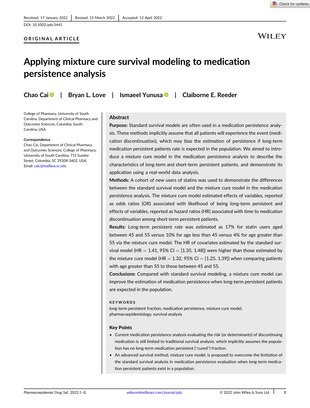
\includegraphics[width=\textwidth]{ref/cai_sm.jpg}};
\end{tikzpicture}
\end{column}
\begin{column}{0.70\contentwidth}
	\begin{itemize}
		\item C.~Cai et al. \textbf{Applying mixture cure survival modeling to medication persistence analysis} \emph{Pharmacoepidemiolol Drug Saf}, 2022;1--8. doi:10.1002/pds5441.
\nocite{cai_applying_2022}
	\end{itemize}
\end{column}
\end{columns}
\end{frame}

\begin{frame}{Recap of survival analysis}
	\begin{itemize}
		\item Time-to-event analysis is fundamental to cohort studies
		\item Unbiased estimates require proper handling of censoring
		\item Kaplan--Meier analysis estimates empirical survival curve
		\item Cox regression allows semiparametric estimation (PH assumption)
	\end{itemize}
\end{frame}

\begin{frame}{Cure survival models}
	\begin{itemize}
		\item Simple survival models consider all cohort members as susceptible
		\begin{itemize}
			\item Good assumption for short follow-up
		\end{itemize}
	\item But if there is a long plateau at the tail of the survival curve
		\begin{itemize}
			\item Evidence for a ``cured'' fraction
		\end{itemize}
	\item \emph{By definition, 100\% of cured cohort members will be censored}
	\end{itemize}
\end{frame}

\begin{frame}{Mixture cure models 1}
\calculatespace%
\begin{columns}
\begin{column}{0.5\contentwidth}
  \centering
  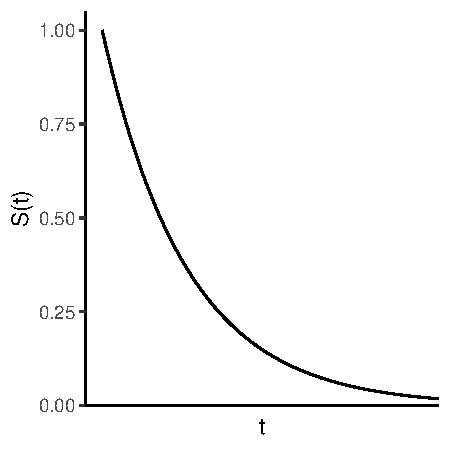
\includegraphics[height=0.7\textheight]{ref/surv1.pdf}

  A bit of this...
\end{column}
\begin{column}{0.5\contentwidth}
  \centering
  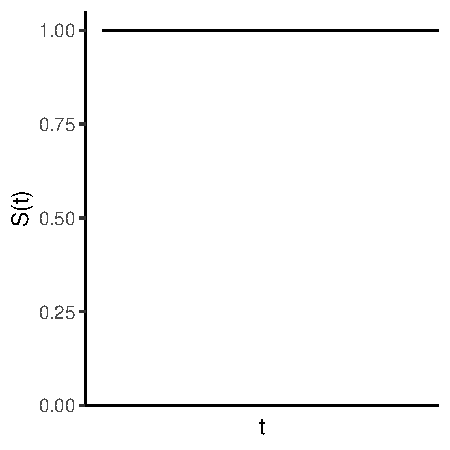
\includegraphics[height=0.7\textheight]{ref/surv2.pdf}

  and a little bit of that
\end{column}
\end{columns}
\end{frame}

\begin{frame}{Mixture cure models 2}
\calculatespace%
\begin{columns}
\begin{column}{0.5\contentwidth}
  \centering
  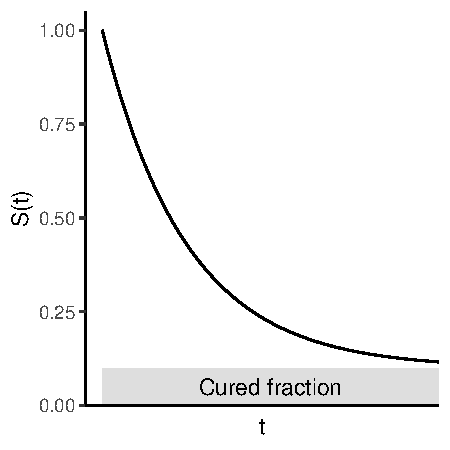
\includegraphics[height=0.7\textheight]{ref/surv3.pdf}
\end{column}
\begin{column}{0.5\contentwidth}
	$S_{pop}(t|X,Z)=\underbrace{\pi(Z)S_u(t|X)}_\text{uncured}+
	\underbrace{1-\pi(Z)}_\text{cured}$
\end{column}
\end{columns}
\end{frame}

%\usebackgroundtemplate{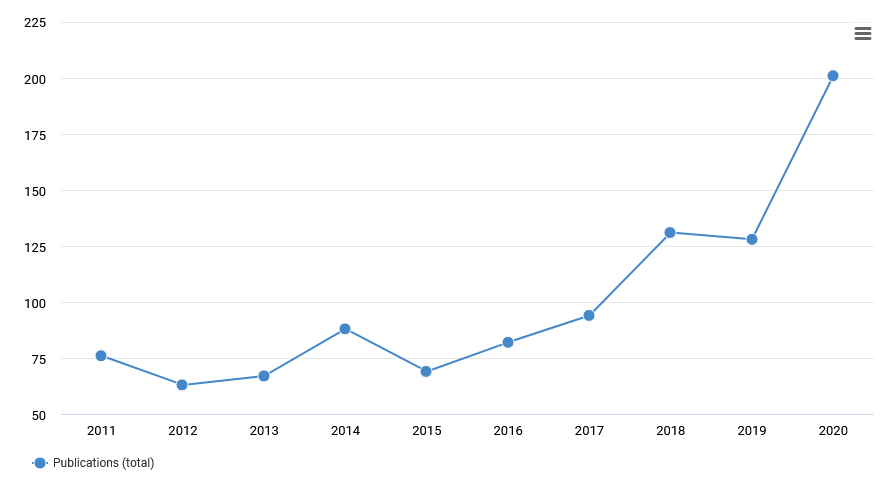
\includegraphics[width=\paperwidth]{ref/newey-west-cites.PNG}}
%\begin{frame}[plain,b]
%\begin{flushright}\texttt{https://app.dimensions.ai/}\end{flushright}
%\end{frame}
%\usebackgroundtemplate{}

\begin{frame}{What's this got to do with medicine persistence?}
	\begin{itemize}
		\item Time-to-event analysis is the obvious way to measure persistence, with discontinuation as the event
		\item Empirically, there may be distinct short- and long-term persistence patterns
		\item In chronic disease, consider the long-term persistent as the ``cured'' fraction
		\item If there is cured fraction, PH assumption is violated
	\end{itemize}
\end{frame}

\begin{frame}{Applying the cure model}
	\begin{itemize}
		\item XXXX
	\end{itemize}
\end{frame}

\begin{frame}{Statistical inference}
    \begin{itemize}
        \item Test if the cured fraction > 0
	\item Test if the follow up is long enough
	\item \emph{n.b. in the Cai et al (2022) paper this is done using parametric models}
    \end{itemize}
\end{frame}

\begin{frame}{Cai et al example 1}
  \centering
  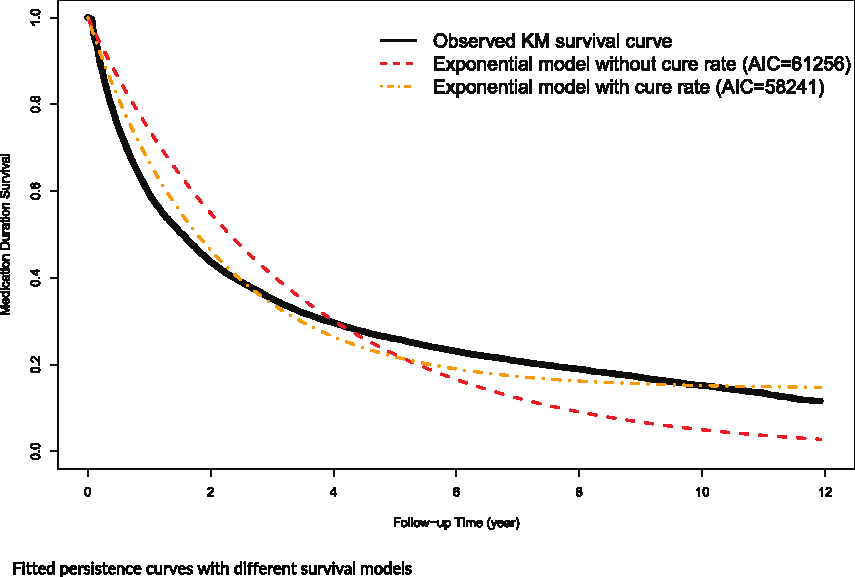
\includegraphics[height=0.7\textheight]{ref/cai_fig2.pdf}
  \flushright{\tiny{\citet{cai_applying_2022}}}
\end{frame}

\begin{frame}{Cai et al example 2}
\calculatespace%
\begin{columns}
\begin{column}{0.5\contentwidth}
  \centering
  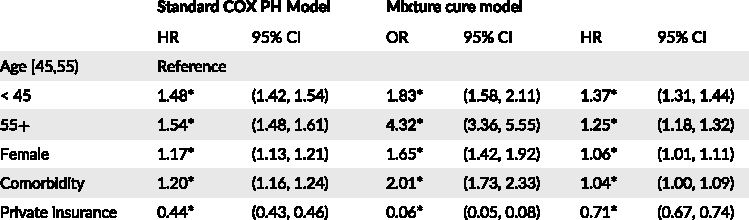
\includegraphics[width=0.9\textwidth]{ref/cai_tab2.pdf}
\end{column}
\begin{column}{0.5\contentwidth}
  \centering
  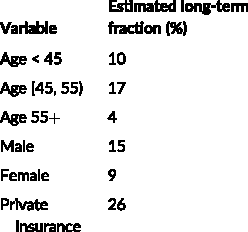
\includegraphics[height=0.6\textheight]{ref/cai_tab3.pdf}
\end{column}
\end{columns}
\flushright{\tiny{\citet{cai_applying_2022}}}
\end{frame}

\begin{frame}{Worked example in R}
\end{frame}

\begin{frame}{The wild west of survival models...}
	\begin{itemize}
		\item There's more to life than just Cox models:
			\begin{itemize}
				\item Parametric survival
				\item Accelerated failure time
				\item Shared/conditional frailty
				\item ...
			\end{itemize}
	\end{itemize}
\end{frame}

\begin{frame}{Summary}
\end{frame}

\begin{frame}{Thanks}
    \begin{itemize}
        \item Andrea
    \end{itemize}
\end{frame}

\begin{frame}{References}
%        \bibliographystyle{apalike}
%        \bibliographystyle{abbrv}
        \tiny\bibliography{cure.bib}
        \bibliographystyle{abbrvnat}
\end{frame}

\end{document}
